% Options for packages loaded elsewhere
\PassOptionsToPackage{unicode}{hyperref}
\PassOptionsToPackage{hyphens}{url}
\PassOptionsToPackage{dvipsnames,svgnames,x11names}{xcolor}
%
\documentclass[
true
]{sn-jnl}

\usepackage{amsmath,amssymb}
\usepackage{iftex}
\ifPDFTeX
  \usepackage[T1]{fontenc}
  \usepackage[utf8]{inputenc}
  \usepackage{textcomp} % provide euro and other symbols
\else % if luatex or xetex
  \usepackage{unicode-math}
  \defaultfontfeatures{Scale=MatchLowercase}
  \defaultfontfeatures[\rmfamily]{Ligatures=TeX,Scale=1}
\fi
\usepackage{lmodern}
\ifPDFTeX\else  
    % xetex/luatex font selection
\fi
% Use upquote if available, for straight quotes in verbatim environments
\IfFileExists{upquote.sty}{\usepackage{upquote}}{}
\IfFileExists{microtype.sty}{% use microtype if available
  \usepackage[]{microtype}
  \UseMicrotypeSet[protrusion]{basicmath} % disable protrusion for tt fonts
}{}
\makeatletter
\@ifundefined{KOMAClassName}{% if non-KOMA class
  \IfFileExists{parskip.sty}{%
    \usepackage{parskip}
  }{% else
    \setlength{\parindent}{0pt}
    \setlength{\parskip}{6pt plus 2pt minus 1pt}}
}{% if KOMA class
  \KOMAoptions{parskip=half}}
\makeatother
\usepackage{xcolor}
\setlength{\emergencystretch}{3em} % prevent overfull lines
\setcounter{secnumdepth}{5}
% Make \paragraph and \subparagraph free-standing
\makeatletter
\ifx\paragraph\undefined\else
  \let\oldparagraph\paragraph
  \renewcommand{\paragraph}{
    \@ifstar
      \xxxParagraphStar
      \xxxParagraphNoStar
  }
  \newcommand{\xxxParagraphStar}[1]{\oldparagraph*{#1}\mbox{}}
  \newcommand{\xxxParagraphNoStar}[1]{\oldparagraph{#1}\mbox{}}
\fi
\ifx\subparagraph\undefined\else
  \let\oldsubparagraph\subparagraph
  \renewcommand{\subparagraph}{
    \@ifstar
      \xxxSubParagraphStar
      \xxxSubParagraphNoStar
  }
  \newcommand{\xxxSubParagraphStar}[1]{\oldsubparagraph*{#1}\mbox{}}
  \newcommand{\xxxSubParagraphNoStar}[1]{\oldsubparagraph{#1}\mbox{}}
\fi
\makeatother


\providecommand{\tightlist}{%
  \setlength{\itemsep}{0pt}\setlength{\parskip}{0pt}}\usepackage{longtable,booktabs,array}
\usepackage{calc} % for calculating minipage widths
% Correct order of tables after \paragraph or \subparagraph
\usepackage{etoolbox}
\makeatletter
\patchcmd\longtable{\par}{\if@noskipsec\mbox{}\fi\par}{}{}
\makeatother
% Allow footnotes in longtable head/foot
\IfFileExists{footnotehyper.sty}{\usepackage{footnotehyper}}{\usepackage{footnote}}
\makesavenoteenv{longtable}
\usepackage{graphicx}
\makeatletter
\newsavebox\pandoc@box
\newcommand*\pandocbounded[1]{% scales image to fit in text height/width
  \sbox\pandoc@box{#1}%
  \Gscale@div\@tempa{\textheight}{\dimexpr\ht\pandoc@box+\dp\pandoc@box\relax}%
  \Gscale@div\@tempb{\linewidth}{\wd\pandoc@box}%
  \ifdim\@tempb\p@<\@tempa\p@\let\@tempa\@tempb\fi% select the smaller of both
  \ifdim\@tempa\p@<\p@\scalebox{\@tempa}{\usebox\pandoc@box}%
  \else\usebox{\pandoc@box}%
  \fi%
}
% Set default figure placement to htbp
\def\fps@figure{htbp}
\makeatother

%%%% Standard Packages

\usepackage{graphicx}%
\usepackage{multirow}%
\usepackage{amsmath,amssymb,amsfonts}%
\usepackage{amsthm}%
\usepackage{mathrsfs}%
\usepackage[title]{appendix}%
\usepackage{xcolor}%
\usepackage{textcomp}%
\usepackage{manyfoot}%
\usepackage{booktabs}%
\usepackage{algorithm}%
\usepackage{algorithmicx}%
\usepackage{algpseudocode}%
\usepackage{listings}%

%%%%

\raggedbottom
\makeatletter
\@ifpackageloaded{caption}{}{\usepackage{caption}}
\AtBeginDocument{%
\ifdefined\contentsname
  \renewcommand*\contentsname{Table of contents}
\else
  \newcommand\contentsname{Table of contents}
\fi
\ifdefined\listfigurename
  \renewcommand*\listfigurename{List of Figures}
\else
  \newcommand\listfigurename{List of Figures}
\fi
\ifdefined\listtablename
  \renewcommand*\listtablename{List of Tables}
\else
  \newcommand\listtablename{List of Tables}
\fi
\ifdefined\figurename
  \renewcommand*\figurename{\textbf{Figure}}
\else
  \newcommand\figurename{\textbf{Figure}}
\fi
\ifdefined\tablename
  \renewcommand*\tablename{\textbf{Table}}
\else
  \newcommand\tablename{\textbf{Table}}
\fi
}
\@ifpackageloaded{float}{}{\usepackage{float}}
\floatstyle{ruled}
\@ifundefined{c@chapter}{\newfloat{codelisting}{h}{lop}}{\newfloat{codelisting}{h}{lop}[chapter]}
\floatname{codelisting}{Listing}
\newcommand*\listoflistings{\listof{codelisting}{List of Listings}}
\captionsetup{labelsep=period}
\makeatother
\makeatletter
\makeatother
\makeatletter
\@ifpackageloaded{caption}{}{\usepackage{caption}}
\@ifpackageloaded{subcaption}{}{\usepackage{subcaption}}
\makeatother

\usepackage[]{natbib}
\bibliographystyle{plainnat}
\usepackage{bookmark}

\IfFileExists{xurl.sty}{\usepackage{xurl}}{} % add URL line breaks if available
\urlstyle{same} % disable monospaced font for URLs
\hypersetup{
  pdftitle={Does the Brain's E:I Balance Really Shape Long-Range Temporal Correlations? Lessons Learned from 3T MRI},
  pdfauthor={, and },
  pdfkeywords={Hurst exponent, long range temporal
correlation, excitatory / inhibitory balance, criticality, complex
systems, visual task, functional magnetic resnonance imaging, magnetic
resonance spectroscopy, functional magnetic resonance spectroscopy},
  colorlinks=true,
  linkcolor={blue},
  filecolor={Maroon},
  citecolor={Blue},
  urlcolor={Blue},
  pdfcreator={LaTeX via pandoc}}


\title[Does the Brain's E:I Balance Really Shape Long-Range Temporal
Correlations? Lessons Learned from 3T MRI]{Does the Brain's E:I Balance
Really Shape Long-Range Temporal Correlations? Lessons Learned from 3T
MRI}

% author setup
\author[1]{\fnm{Lydia} \sur{Sochan}}\email{lydiasochan@gmail.com}\author*[1,2,3]{\fnm{Alexander Mark} \sur{Weber}}\email{aweber@bcchr.ca}
% affil setup
\affil[1]{, \orgname{School of Biomedical Engineering, The University of
British Columbia, Vancouver, BC, Canada}}
\affil[2]{, \orgname{BC Children's Hospital Research Institute, The
University of British Columbia, Vancouver, BC, Canada}}
\affil[3]{, \orgname{Pediatrics, The University of British Columbia,
Vancouver, BC, Canada}}

% abstract 


% keywords
\keywords{Hurst exponent,  long range temporal correlation,  excitatory
/ inhibitory balance,  criticality,  complex systems,  visual
task,  functional magnetic resnonance imaging,  magnetic resonance
spectroscopy,  functional magnetic resonance spectroscopy}

\begin{document}
\maketitle


\textsuperscript{1} School of Biomedical Engineering, The University of
British Columbia, Vancouver, BC, Canada\\
\textsuperscript{2} BC Children's Hospital Research Institute, The
University of British Columbia, Vancouver, BC, Canada\\
\textsuperscript{3} Pediatrics, The University of British Columbia,
Vancouver, BC, Canada

\textsuperscript{*} Correspondence:
\href{mailto:aweber@bcchr.ca}{Alexander Mark Weber
\textless{}aweber@bcchr.ca\textgreater{}}

\subsection*{Abstract}\label{abstract}
\addcontentsline{toc}{subsection}{Abstract}

A 3T multimodal MRI study of healthy adults (n=19; 10 female; 21.3 -
53.4 years) was performed to investigate the potential link between fMRI
long-range temporal correlations and excitatory/inhibitory balance. The
study objective was to determine if the Hurst exponent (H) --- an
estimate of the self-correlation and signal complexity --- of the
blood-oxygen-level-dependent signal is correlated with the
excitatory-inhibitory (E:I) ratio. E:I has been proposed to serve as a
control parameter for brain criticality, which H is believed to be a
measure of. Thus, understanding if H and E:I are correlated would serve
to clarify this relationship. Moreover, findings in this domain have
implications for neurological and neuropsychiatric conditions with
disrupted E:I balance, such as autism spectrum disorder, schizophrenia,
and Alzheimer's disease. From a practical perspective, H is easier to
accurately measure than E:I ratio at 3T MRI. If H can serve as a proxy
for E:I, it may serve as a more useful clinical biomarker for this
imbalance and for neuroscience research in general. The study collected
functional MRI and magnetic resonance spectroscopy data during rest and
movie-watching. H was found to increase with movie-watching compared to
rest, while E:I did not change between conditions. H and E:I were not
correlated during either movie-watching or rest. This study represents
the first attempt to investigate this connection \emph{in vivo} in
humans. We conclude that, at 3T and with our particular methodologies,
no association was found. We end with lessons learned and suggestions
for future research.

\section{Introduction}\label{introduction}

The brain is composed of individual neurons, each
computationally-limited, that ultimately work together to produce
astonishingly complex operations. Understanding how these neurons
produce this emergent behaviour remains one of the great scientific
challenges of our time. Recent advances in neuroscience have led to the
emergence of the Critical Brain Hypothesis, which posits that the brain
operates at a critical point, a state where order and disorder are
balanced to enable the most efficient information processing
\citep{decoRestingBrainsNever2013, beggsBeingCriticalCriticality2012, barangerChaosComplexityEntropy2000, bassettUnderstandingComplexityHuman2011, zimmernWhyBrainCriticality2020, liangExcitationInhibitionBalance2024, poilCriticalStateDynamicsAvalanches2012, lombardiBalanceExcitationInhibition2017, baumgartenCriticalExcitationinhibitionBalance2019, bruiningMeasurementExcitationinhibitionRatio2020, trakoshisIntrinsicExcitationinhibitionImbalance, gaoInferringSynapticExcitation2017, tianTheoreticalFoundationsStudying2022, rubinovNeurobiologicallyRealisticDeterminants2011}.
When in a critical state, the brain is optimally responsive to both
internal and external stimuli while maintaining a balance between
stability and instability
\citep{decoRestingBrainsNever2013, beggsBeingCriticalCriticality2012, tianTheoreticalFoundationsStudying2022, rubinovNeurobiologicallyRealisticDeterminants2011}.
A fundamental theorem proposing how neural networks achieve this
delicate balance centers around the excitation-inhibition (E:I) ratio:
the balance of excitatory and inhibitory neural activity, often
operationalized as the ratio of the primary excitatory and inhibitory
neurotransmitters (i.e.~glutamate (Glu) and \(\gamma\)-aminobutyric acid
(GABA)
\citep{liangExcitationInhibitionBalance2024, lombardiBalanceExcitationInhibition2017, baumgartenCriticalExcitationinhibitionBalance2019, bruiningMeasurementExcitationinhibitionRatio2020, trakoshisIntrinsicExcitationinhibitionImbalance, gaoInferringSynapticExcitation2017}).

\emph{In vivo} measurement of brain criticality can be achieved using
several available methods, as systems near a critical state often
exhibit fractal-like fluctuations or scale-invariance
\citep{munozColloquiumCriticalityDynamical2018}. Scale-invariance has
been observed extensively across various neuronal spatio-temporal
scales, from dendritic branching structures
\citep{casertaDeterminationFractalDimension1995} in the spatial domain,
to neurotransmitter release
\citep{lowenQuantalNeurotransmitterSecretion1997}, neuronal firing rates
\citep{mazzoniDynamicsSpontaneousActivity2007}, local field potentials
\citep{bedardMacroscopicModelsLocal2009}, electroencephalography (EEG)
\citep{bullmoreFractalAnalysisElectroencephalographic1994} and
functional magnetic resonance imaging (fMRI), which measures the blood
oxygen level-dependent (BOLD) signal
\citep{zarahnEmpiricalAnalysesBOLD1997, fadiliWaveletGeneralizedLeastSquares2002, campbellMonofractalAnalysisFunctional2022}
in the time domain. This fractal structure can be quantified by
assessing the signal's long-range temporal correlations (LRTC), which
reflect the persistence or memory in a time series, where future values
are statistically related to past values over long extended periods. The
Hurst exponent (H) is a useful measure for evaluating LRTC
\citep{ekeFractalCharacterizationComplexity2002, campbellMonofractalAnalysisFunctional2022}.
An H value between 0.5 and 1 indicates a long-range positive
correlation, with large values being followed by large values and small
values by small ones. Conversely, an H exponent value between 0 and 0.5
indicates a long-range negative correlation, where large values are
likely to be followed by small ones and vice versa. An H value of 0.5 is
uncorrelated random noise.

H has emerged as a valuable tool in neuroscience and clinical research.
Typically, H values reported in adult brains are above 0.5, with higher
H values in grey matter than white matter or cerebrospinal fluid
\citep{dongHurstExponentAnalysis2018, winkMonofractalMultifractalDynamics2008}.
Some key findings from neuroscience research include: a decrease in H
during task performance
\citep{ciuciuInterplayFunctionalConnectivity2014, heScaleFreePropertiesFunctional2011},
negative correlations with task novelty and difficulty
\citep{churchillSuppressionScalefreeFMRI2016}, increases with age in the
frontal and parietal lobes \citep{dongHurstExponentAnalysis2018}, and
hippocampus \citep{winkAgeCholinergicEffects2006}, but decreases with
age in the insula, and limbic, occipital and temporal lobes
\citep{dongHurstExponentAnalysis2018}, and more
\citep{campbellMonofractalAnalysisFunctional2022}. In terms of clinical
findings, abnormal H values have been identified in Alzheimer's disease
(AD)
\citep{maximFractionalGaussianNoise2005, warsiCorrelatingBrainBlood2012},
autism spectrum disorder (ASD)
\citep{donaTemporalFractalAnalysis2017, laiShiftRandomnessBrain2010},
mild traumatic brain injury \citep{donaFractalAnalysisBrain2017}, major
depressive disorder
\citep{weiIdentifyingMajorDepressive2013, jingIdentifyingCurrentRemitted2017}
and schizophrenia \citep{sokunbiNonlinearComplexityAnalysis2014}.
Crucially, these same disorders have been associated with imbalances in
E:I (AD:
\citep{lauterbornIncreasedExcitatoryInhibitory2021, vicovarelaExcitatoryinhibitoryImbalanceAlzheimers2019};
ASD
\citep{sohalExcitationinhibitionBalanceFramework2019, uzunovaExcitatoryInhibitoryImbalance2016, bruiningMeasurementExcitationinhibitionRatio2020};
depression \citep{pagePrefrontalExcitatoryInhibitory2019}; and
schizophrenia \citep{kangInterplayMentalDisorder2019})

In addition to its implications for the critical brain hypothesis,
establishing a connection between E:I and H could facilitate simpler
estimation of excitatory and inhibitory neurotransmitters, as precise
measurement of E:I is technically challenging
\citep{ajramContribution1HMagnetic2019}. Currently, magnetic resonance
spectroscopy (MRS) is the only non-invasive method for \emph{in vivo}
assessment of the Glu/GABA ratio (excitatory to inhibitory
neurotransmitters) in humans
\citep{stanleyFunctionalMagneticResonance2018, harrisEdited1Magnetic2017}.
Unfortunately, MRS suffers from limited spatial and temporal resolution
\citep{gaoInferringSynapticExcitation2017, ajramContribution1HMagnetic2019, stanleyFunctionalMagneticResonance2018}.
If H could function as a substitute for E:I, it would simplify the
estimation of E:I in conditions of interest such as ASD, AD, and
schizophrenia.

Going beyond clinical observations that imply a link between H and E:I,
several studies have attempted to explore this association directly.
However, they have primarily relied on computational models or animal
studies
\citep{liangExcitationInhibitionBalance2024, poilCriticalStateDynamicsAvalanches2012, lombardiBalanceExcitationInhibition2017, baumgartenCriticalExcitationinhibitionBalance2019, bruiningMeasurementExcitationinhibitionRatio2020, trakoshisIntrinsicExcitationinhibitionImbalance, gaoInferringSynapticExcitation2017}.
To date, no \emph{in vivo} study has validated this association in
humans. Moreover, the existing research findings have so far been
inconsistent, with some reporting positive-linear, negative-linear, or
U-shaped relationships between the two variables. Therefore, further
investigation is needed to establish the true nature of the potential
E:I-Hurst relationship and to confirm its presence within the human
brain. The current study aimed to explore the potential E:I-Hurst
relationship in vivo , specifically within the visual cortex during
movie-watching and resting periods.

\section{Methods}\label{methods}

\subsection{Participants}\label{participants}

Twenty-seven healthy adult participants were recruited to the study. One
participant was not scanned due to feelings of claustrophobia while in
the scanner. After our analysis and performing quality assurance (see
below), a further seven participants were removed for having less than
ideal MRI data quality, leaving nineteen final participants, between the
ages of 21.3 and 53.4 (mean age ± sd: 30.1 ± 8.7 years; 9 males).

\subsection{Ethics Statement}\label{ethics-statement}

Written informed consent was obtained from all participants. Ethics
approval was granted by the Clinical Research Ethics Board at the
University of British Columbia and BC Children's \& Women's Hospital
(H21-02686).

\subsection{Scanning Procedure}\label{scanning-procedure}

After two anatomical sequences were acquired, participants were
instructed to visually fixate on a cross-hair for 24 minutes. During
this period, an fMRI, single-voxel semi Localization by Adiabatic
SElective Refocusing (sLASER)
\citep{ozShortechoSingleshotFullintensity2011}, and single-voxel
MEscher-Garwood Point-REsolved SpectroScopy (MEGA-PRESS)
\citep{mescherSimultaneousVivoSpectral1998} sequences were acquired (see
Figure~\ref{fig-method} A and Section~\ref{sec-mriacq}). Next,
participants were instructed to watch a nature documentary (Our Planet
(2019), Episode 3, ``Jungles'' \citet{cordeyJungles2019}) for 24
minutes. During this period, another set of fMRI, sLASER, and MEGA-PRESS
sequences were acquired. See Figure~\ref{fig-method} B for a visual
representation of the scanning protocol. Total scan duration was
approximately 1 hour. All participants followed the same order of rest
than movie, and all participants saw the same movie segment, beginning
at the same time during the scan.

\phantomsection\label{cell-fig-method}
\begin{figure}[H]

\centering{

\pandocbounded{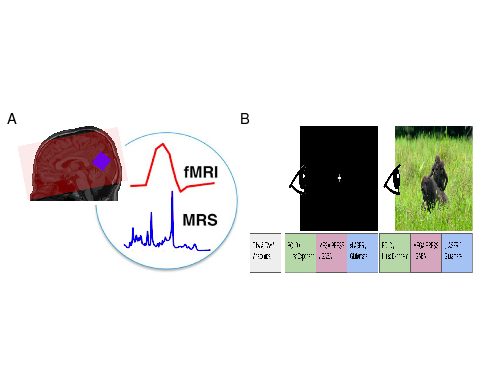
\includegraphics[keepaspectratio]{index_files/figure-pdf/fig-method-1.pdf}}

}

\caption{\label{fig-method}\textbf{Overview of the MRI acquisition
protocol.} A) fMRI coverage was across the whole-brain (example coverage
in red). MRS voxels were placed in the visual cortex (blue). Background
image is of a T1w acquisition from a sample subject. B) fMRI, MEGA-PRESS
and sLASER were acquired first with participants looking at a white
cross for 24 mintues. Next, the same sequences were acquired with the
participants viewing a nature documentary for an identical period of
time.}

\end{figure}%

\subsection{Acquisition Details}\label{sec-mriacq}

Scans were performed at BC Children's Hospital MRI Research Facility on
a 3.0 Tesla GE Discovery MR750 scanner (scanner software version:
DV26.0\_R03) with a Nova Medical 32 channel head coil. Participants
changed into scrubs and were screened by an MRI technologist.
Participants were given wax earplugs and a fiducial was placed on their
left temple. Participants were provided with an audio headset and
blanket once lying down on the scanner bed. Since visual stimuli were to
be rear-projected, position and angle of mirror above patient eyes was
adjusted for optimal movie viewing.

The following MRI scans were acquired. A 3D T1-weighted sagittal fast
spoiled gradient echo (FSPGR) sequence; a 3D T2-weighted sagittal CUBE;
a 2D echo-planar imaging (EPI) multi-echo gradient-echo fMRI sequence; a
MEGA-PRESS sequence; and an sLASER sequence. Details are listed in
Table~\ref{tbl-mriacq}.

\begin{longtable}[]{@{}
  >{\raggedright\arraybackslash}p{(\linewidth - 16\tabcolsep) * \real{0.1844}}
  >{\raggedright\arraybackslash}p{(\linewidth - 16\tabcolsep) * \real{0.0838}}
  >{\raggedright\arraybackslash}p{(\linewidth - 16\tabcolsep) * \real{0.0670}}
  >{\raggedright\arraybackslash}p{(\linewidth - 16\tabcolsep) * \real{0.0670}}
  >{\raggedright\arraybackslash}p{(\linewidth - 16\tabcolsep) * \real{0.0894}}
  >{\raggedright\arraybackslash}p{(\linewidth - 16\tabcolsep) * \real{0.1229}}
  >{\raggedright\arraybackslash}p{(\linewidth - 16\tabcolsep) * \real{0.1564}}
  >{\raggedright\arraybackslash}p{(\linewidth - 16\tabcolsep) * \real{0.2067}}
  >{\raggedright\arraybackslash}p{(\linewidth - 16\tabcolsep) * \real{0.0223}}@{}}
\caption{\textbf{Summary of MRI acquisition details} TE = echo time; TR
= repetition time; FOV = field of view; FSPGD = fast spoiled
gradient-echo; CUBE = a GE acronym; EPI = echo-planar imaging; fMRI =
functional magnetic resonance imaging; sLASER = semi localization by
adiabatic selective refocusing; MEGA-PRESS = Mescher-Garwood
point-resolved spectroscopy}\label{tbl-mriacq}\tabularnewline
\toprule\noalign{}
\begin{minipage}[b]{\linewidth}\raggedright
Sequence
\end{minipage} & \begin{minipage}[b]{\linewidth}\raggedright
TE (ms)
\end{minipage} & \begin{minipage}[b]{\linewidth}\raggedright
TR (ms)
\end{minipage} & \begin{minipage}[b]{\linewidth}\raggedright
Flip Angle
\end{minipage} & \begin{minipage}[b]{\linewidth}\raggedright
FOV
\end{minipage} & \begin{minipage}[b]{\linewidth}\raggedright
Slice Thickness (mm)
\end{minipage} & \begin{minipage}[b]{\linewidth}\raggedright
In-Plane Resolution (mm²)
\end{minipage} & \begin{minipage}[b]{\linewidth}\raggedright
Other Parameters
\end{minipage} & \begin{minipage}[b]{\linewidth}\raggedright
Time (mins)
\end{minipage} \\
\midrule\noalign{}
\endfirsthead
\toprule\noalign{}
\begin{minipage}[b]{\linewidth}\raggedright
Sequence
\end{minipage} & \begin{minipage}[b]{\linewidth}\raggedright
TE (ms)
\end{minipage} & \begin{minipage}[b]{\linewidth}\raggedright
TR (ms)
\end{minipage} & \begin{minipage}[b]{\linewidth}\raggedright
Flip Angle
\end{minipage} & \begin{minipage}[b]{\linewidth}\raggedright
FOV
\end{minipage} & \begin{minipage}[b]{\linewidth}\raggedright
Slice Thickness (mm)
\end{minipage} & \begin{minipage}[b]{\linewidth}\raggedright
In-Plane Resolution (mm²)
\end{minipage} & \begin{minipage}[b]{\linewidth}\raggedright
Other Parameters
\end{minipage} & \begin{minipage}[b]{\linewidth}\raggedright
Time (mins)
\end{minipage} \\
\midrule\noalign{}
\endhead
\bottomrule\noalign{}
\endlastfoot
3D T1-weighted FSPGR & 2.176 & 7.216 & 12 & 256 × 256 & 0.9 & 0.9375 ×
0.9375 & - & 5 \\
3D T2-weighted CUBE & 75.242 & 2,504.0 & 90 & 256 x 256 & 0.9 & 0.9375 ×
0.9375 & - & 4 \\
2D EPI Multi-Echo fMRI & 12.2, 35.352, 58.504 & 1,500 & 52 & 64 x 64 &
3.6 & 3.5938 × 3.5938 & Acceleration factor = 6 & 12 \\
MEGA-PRESS & 68 & 1,800 & 90 & - & 28.0 & 28.0 x 28.0 & - & 4 \\
sLASER & 35 & 2,000 & 90 & - & 28.0 & 28.0 x 28.0 & - & 8 \\
\end{longtable}

For both MRS sequences, the voxel size was set to 2.8 x 2.8 x 2.8
cm\textsuperscript{3}. MRS voxels were rotated and placed in the
occipital lobe, aligned along the calcarine fissure. Finally, blip-up
and blip-down spin-echo versions of the fMRI sequence were acquired at
the end to estimate the B0 non-uniformity map for fMRI phase distortion
correction.

\subsection{Image Processing}\label{image-processing}

Our full image processing pipeline has been can be accessed from our
Github account page:
\href{https://github.com/WeberLab/EI_Hurst_Analysis}{github.com/WeberLab/EI\_Hurst\_Analysis}

Images were downloaded offline from the scanner in raw Digital Imaging
and Communications in Medicine (DICOM) format. DICOM files were then
converted to Neuroimaging Informatics Technology Initiative (NIfTI)
using Chris Rorden's \texttt{dcm2niix}
\citep{liFirstStepNeuroimaging2016} (v1.0.20211006) and then to Brain
Imaging Data Structure (BIDS) \citep{gorgolewskiBrainImagingData2016}
format using \texttt{dcm2bids} \citep{boreDcm2Bids2023} (v2.1.6).

\subsubsection{Structural Images}\label{structural-images}

The T1w image was corrected for intensity non-uniformity with
\texttt{N4BiasFieldCorrection} \citep{tustisonN4ITKImprovedN32010} and
distributed using \texttt{ANTs}
\citep{avantsSymmetricDiffeomorphicImage2008} (v2.3.335) to be used as a
T1w-reference for the rest of the workflow. The T1w-reference was
skull-stripped using a \texttt{Nipype}
\citep{gorgolewskiNipypeFlexibleLightweight2016} implementation of
\texttt{antsBrainExtraction.sh} from \texttt{ANTs}; \texttt{OASIS30ANTs}
was used as a target template. \texttt{Fast}
\citep{zhangSegmentationBrainMR2001} (\texttt{FSL}
\citep{smithAdvancesFunctionalStructural2004} v.6.0.5.1:57b01774, RRID:
SCR\_002823) was used for brain tissue segmentation into cerebrospinal
fluid (CSF), white matter (WM), and gray matter (GM). Brain surfaces
were reconstructed with \texttt{recon-all}
\citep{daleCorticalSurfacebasedAnalysis1999} (\texttt{FreeSurfer}
\citep{daleCorticalSurfacebasedAnalysis1999} 7.3.2, RRID: SCR\_001847).
The previously-estimated brain mask was refined with \texttt{Mindboggle}
\citep{kleinMindbogglingMorphometryHuman2017} (RRID:SCR\_002438) to
reconcile ANTs-derived and FreeSurfer-derived segmentations of cortical
GM. \texttt{AntsRegistration}
\citep{avantsSymmetricDiffeomorphicImage2008} (\texttt{ANTs} 2.3.3) was
used to perform volume-based spatial normalization to two standard
spaces: MNI152NLin2009cAsym and MNI152NLin6Asym. Normalization used
brain-extracted versions of both T1w reference and T1w template.

\subsubsection{fMRI}\label{fmri}

Using \texttt{fMRIPrep} \citep{estebanFMRIPrepRobustPreprocessing2019},
the shortest echo of the BOLD run was used to generate a reference
volume (both skull-stripped and skull-included). Head-motion parameters
with respect to the BOLD reference (transformation matrices as well as
six corresponding rotation and translation parameters) were estimated
before spatiotemporal filtering using \texttt{mcflirt}
\citep{jenkinsonImprovedOptimizationRobust2002} (\texttt{FSL}
v6.0.5.1:57b01774). The fieldmap was aligned with rigid registration to
the target EPI reference run. Field coefficients were mapped to the
reference EPI using the transform. BOLD runs were slice-time corrected
to 643 ms (half of slice acquisitio range of 0-1290 ms) using
\texttt{3dTshift} from \texttt{AFNI} \citep{coxAFNISoftwareAnalysis1996}
(RRIS: SCR\_005927). To estimate T2* map from preprocessed EPI echoes, a
voxel-wise fitting was performed by fitting the maximum number of echoes
with reliable echoes in a particular voxel to a monoexponential signal
decay model with nonlinear regression. Initial values were T2\emph{/S0
estimates from a log-linear regression fit. This calculated T2} map was
then used to optimally combine preprocessed BOLD across echoes using the
method by Posse et al.~(1999)
\citep{posseEnhancementBOLDcontrastSensitivity1999}. The generated BOLD
reference was then co-registered (6 degrees of freedom) to the T1w
reference with \texttt{bbregister} (\texttt{FreeSurfer}
\citep{daleCorticalSurfacebasedAnalysis1999}) using boundary-based
registration. First, a reference volume and its skull-stripped
equivalent were generated with \texttt{fMRIPrep}. Confounding time
series were calculated from preprocessed BOLD: framewise displacement
(FD), DVARS, and three region-wise global signals. \texttt{Tedana}
\citep{dupreTEdependentAnalysisMultiecho2021} was then used to denoise
the data by decomposing the multi-echo BOLD data via principal component
analysis (PCA) and independent component analysis (ICA). The resulting
components are automatically analyzed to determine whether they are
TE-dependent or -independent. TE-dependent components were classified as
BOLD, while TE-independent components were classified as non-BOLD and
were discarded as part of data cleaning.

Participants were excluded from further ananlysis if their mean FD was
\textgreater{} 0.15 mm.

\subsection{MRS}\label{mrs}

sLASER data were processed and fit to a spectrum using \texttt{Osprey}
\citep{oeltzschnerOspreyOpenSourceProcessing2020} (v2.4.0). Full width
half-maximum (FWHM) of the single-Lorentzian fit of the
N-acetylaspartate (NAA) peak were calculated for quality assurance
purposes. The MRS voxel was co-registered to T1w reference image and
segmented by \texttt{SPM12}
\citep{fristonStatisticalParametricMapping2007} into CSF, GM, and WM.
Metabolites were water-scaled as well as tissue- and
relaxation-corrected by the Gasparovic et al.~(2006) method
\citep{gasparovicUseTissueWater2006}. Glutamate is challenging to
capture due to its signal overlaps with other metabolites
\citep{pasantaFunctionalMRSStudies2023}. In particular, Glu shares a
similar chemical structure with glutamine (Gln) which causes the
spectral features of Glu to be contaminated with Gln
\citep{ramadanGlutamateGlutamineReview2013}. As a result, we decided to
report Glx values, which co-reports Glu and Gln to avoid errors in
spectral assignment, especially since it is controversial whether Glu
can reliably be separated from Gln at 3T
\citep{pasantaFunctionalMRSStudies2023, ramadanGlutamateGlutamineReview2013}.
We henceforth refer to Glu as either Glx.

MEGA-PRESS data were processed and fit with \texttt{Osprey}, and were
relaxation-, tissue- and alpha-corrected using the Harris et al.~(2015)
method \citep{harrisSpectralEditingMeasurementsGABA2015}.
\texttt{Osprey} values were ultimately used for further analysis. Due to
the J-editing sequence of MEGA-PRESS, a challenge of GABA quantification
is macromolecule quantification
\citep{harrisSpectralEditingMeasurementsGABA2015}. As a result, we
report GABA+, a measure which co-reports GABA with macromolecules.
Macromolecules (MM) are expected to account for approximately 45\% of
the GABA+ signal \citep{harrisSpectralEditingMeasurementsGABA2015}.
While a macromolecule-suppressed estimate of GABA seems ideal, a recent
25-site and multi-vendor study conducted at 3T found that GABA+ showed
much lower coefficient of variation than MM-suppressed GABA, meaning
that GABA+ is more consistent across research sites and MRI vendors
(i.e., Philips, GE, Siemens) \citep{mikkelsenBigGABAII2019}. Moreover,
GABA+ shows greater reliability for both creatine-referenced and
water-suppressed estimates
\citep{mikkelsenBigGABAEdited2017, mikkelsenBigGABAII2019}. MM-supressed
GABA and GABA+ estimates are also correlated, albeit weakly- to
moderately-so
\citep{harrisSpectralEditingMeasurementsGABA2015, mikkelsenBigGABAII2019, mikkelsenBigGABAEdited2017}.
Consequently, we report GABA+ to allow for easier comparison of our
results to other studies as well as reproducibility.

Basis sets were created using \texttt{MRSCloud}
\citep{huiMRSCloudCloudbasedMRS2022, moriMRICloudDeliveringHighThroughput2016}.
For sLASER, `localization' was set to `sLASER', `vendor' to `GE',
`editing' to `UnEdited', and `TE' to 35. For MEGA-PRESS, `localization'
was set to `PRESS', `editing' to `MEGA', `TE' to 68, `edit on' to `1.9',
`edit off' to `7.5', and `pulse duration' to `14'. Metabolites included
for both basis sets were: Asc, Asp, Cr, CrCH2, EA, GABA, GPC, GSH, Gln,
Glu, Gly, H2O, Lac, NAA, NAAG, PCh, PCr, PE, Ser, Tau, mI, and sI.
Excitatory-inhibitory ratio (E:I) was calculated as {[}Glx in
i.u.{]}/{[}GABA+ in i.u.{]}, a common practice to report E:I using MRS
\citep{rideauxNoBalanceGlutamate+glutamine2021}.

Participants were excluded from further analysis if any of their MRS
scans had FWHM \textgreater{} 10. Originally we intended to calculate,
report and analyze MRS as tissue-corrected quantitative values. However,
the \texttt{Osprey} software was reporting Glx values that were an order
of magnitude larger than reported values in the literature. Despite
several attempts, we were unable to locate the source of this error.
Therefore we decided to use metabolite to creatine ratios (i.e.~Glx /
tCr and GABA+ / tCr) to be safe.

\subsection{Hurst Exponent
Calculation}\label{hurst-exponent-calculation}

Hurst exponent was calculated from the power spectrum density (PSD) of
the BOLD signal. A log-log plot was used, where log power was plotted
against log frequency; generally, if a log-log plot results in a linear
relationship, it is assumed that the mean slope of this line represents
the power-law exponent \citep{zimmernWhyBrainCriticality2020}. A PSD
shows the distribution of signal variance (`power') across frequencies.
Complex signals are classified into two categories: fractional Gaussian
noise (fGn) and fractional Brownian motion (fBm)
\citep{duffPowerSpectralDensity2008, ekeFractalCharacterizationComplexity2002}.
The former is a stationary signal (i.e., does not vary over time), while
the latter is non-stationary with stationary increments
\citep{ekeFractalCharacterizationComplexity2002}. Most physiological
signals consist of fBm, but fMRI BOLD is typically conceptualized as fGn
once motion-corrected; otherwise put, unprocessed BOLD signal is
initially fBm which is converted to fGn with appropriate processing
\citep{bullmoreWaveletsFunctionalMagnetic2004}. fBm and fGn require
distinct H calculation methods
\citep{ekeFractalCharacterizationComplexity2002}. PSD was estimated
using Welch's method \citep{welchUseFastFourier1967} from the Python
\texttt{Scipy.Signal} library \citep{virtanenSciPy10Fundamental2020}.
Data were divided into 8 windows of 50\% overlap and averaged. The
spectral index, , was calculated from the full frequency spectrum. The
spectral index was then converted to H using the following equation
\citep{ekeFractalCharacterizationComplexity2002, schaeferComparativeAnalysisSpectral2014}:

\[
H = \frac{1 + \beta}{2}
\]

Since it cannot be assumed that all fBm is removed from the signal, we
use the concept of `extended Hurst' (H') in this study: for 0
\textless{} H \textless{} 1, the signal is understood as fGn, while for
1 \textless{} H \textless{} 2, the signal is assumed to be fBm
\citep{campbellFractalBasedAnalysisFMRI2022}. More generally, it is also
assumed that when 0.5 \textless{} H \textless{} 1.5, the signal displays
1/f behaviour \citep{zimmernWhyBrainCriticality2020}.H was calculated
for all voxels in the brain of each subject. A brain mask was then
applied which included only GM and the region of the MRS voxel in the
visual cortex. H was averaged across the brain mask area, using only
non-zero voxels.

\subsection{Statistics}\label{statistics}

All statistical analyses were performed using \texttt{R}
\citep{rcoreteamLanguageEnvironmentStatistical2021} and \texttt{RStudio}
(v2023.06.0+421). Difference of means between rest and movie conditions
were calculated using paired Student's t-tests
\citep{studentProbableErrorMean1908}. Correlations were calculated using
Pearson's method \citep{freedmanStatistics2007}. Finally, linear
mixed-effect models were used to test for more complicated models.

\section{Results}\label{results}

\subsection{Participant Demographics}\label{participant-demographics}

Twenty-seven participants were originally recruited for the study.
Twenty-six of these participants were successfully scanned, but one
participant experienced anxiety and chose not to continue. Of the
remaining 26 participants, 19 were included in the final analysis: two
were removed due to low MRS quality (FWHM \textgreater{} 10) and five
were removed due to low fMRI quality (mean FD \textgreater{} 0.15 mm).
See Figure~\ref{fig-partflow}.

\begin{figure}

\centering{

\pandocbounded{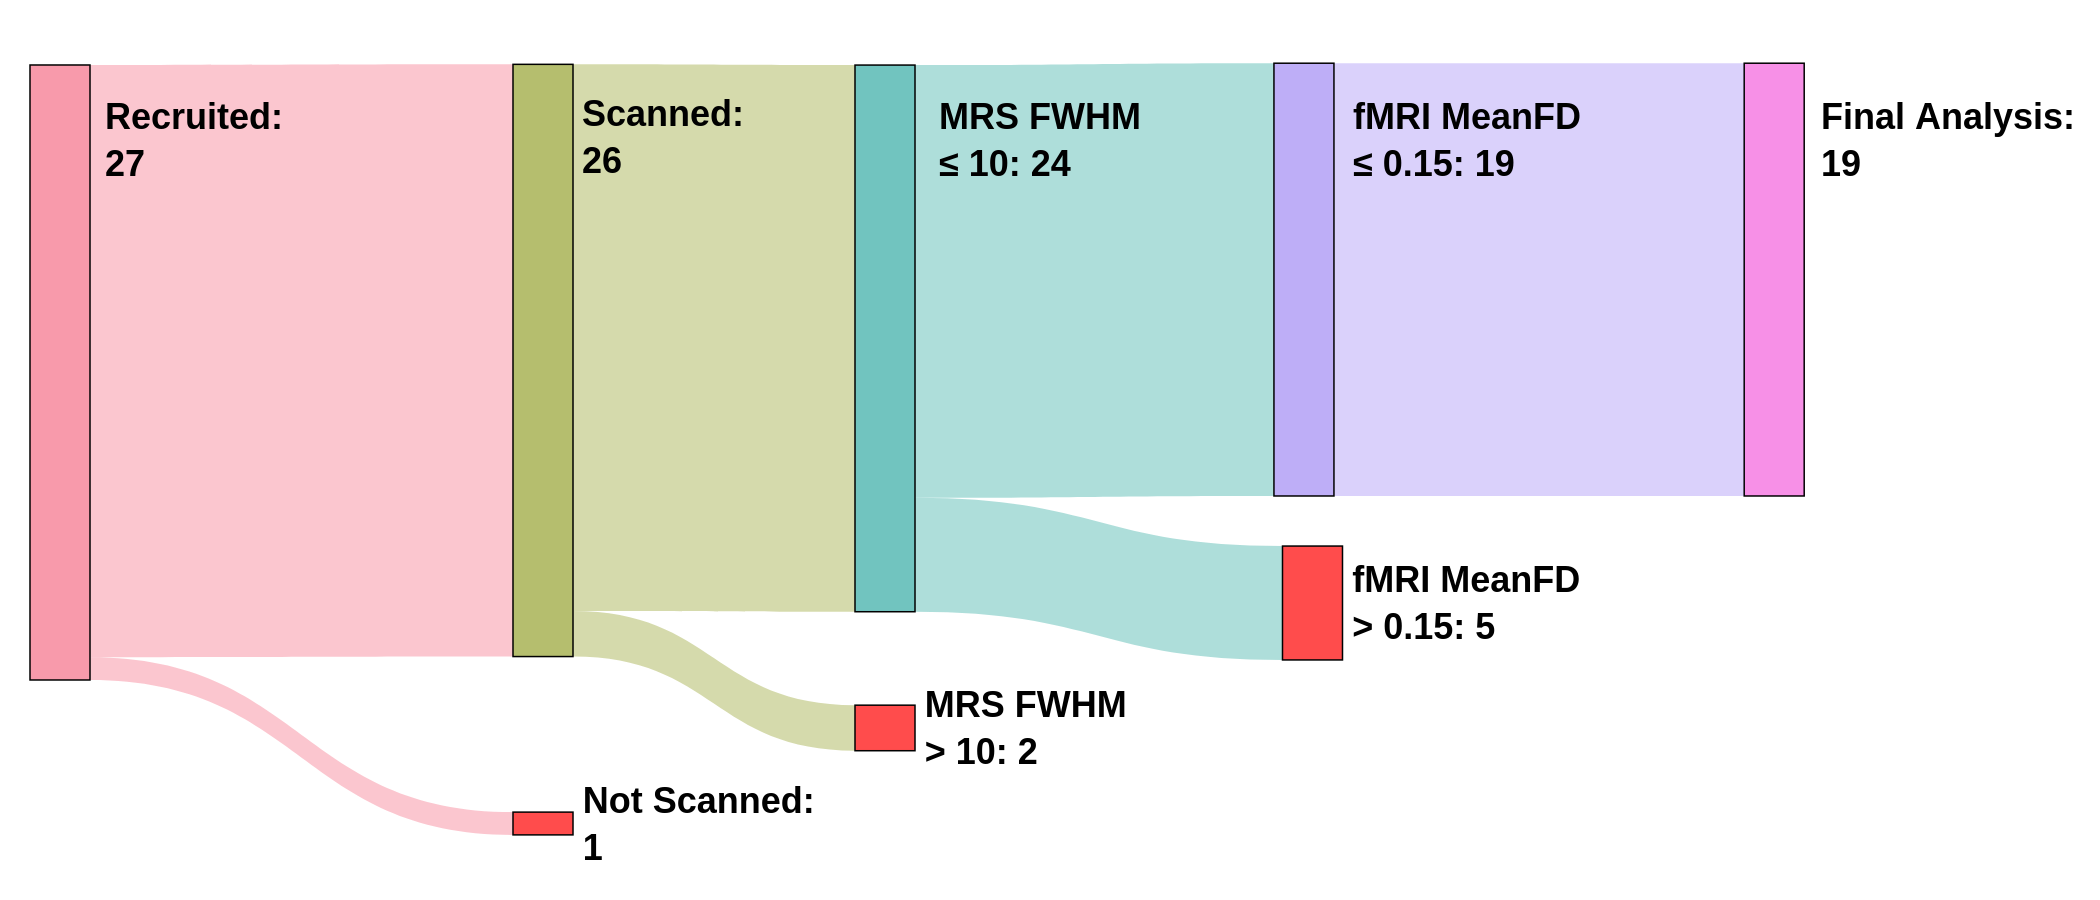
\includegraphics[keepaspectratio]{./images/ParticipantFlow.png}}

}

\caption{\label{fig-partflow}\textbf{Flowchart of participant,
recruitment, scanning and exclusion}. The number of participants at each
stage is indicated within each node. Participants were excluded based on
MRS FWHM and fMRI Mean FD thresholds, resulting in 19 participants
included in the final analysis}

\end{figure}%

The final study sample included 9 males and 10 females between ages 21.3
and 53.4, with a mean age and standard deviation of 30.1 ± 8.7 years.

\subsection{Data Quality}\label{data-quality}

After exclusion, FWHM (mean ± sd) at rest in sLASER and MEGAPRESS were
8.52 ± 0.7 and 7.02 ± 0.7, respectively. During movie watching, FWHM in
sLASER and MEGAPRESS were 8.37 ± 0.65 and 6.98 ± 0.86.

Glx and GABA+ were tested for associations with FWHM values during rest
and movie watching. Glx during rest was found to be negatively
correlated with FWHM (r = -0.53, p = 0.02). No other correlations were
significant.

An average of all MRS voxel placements can be seen in
Figure~\ref{fig-mrsquality} A, and a sample of the \texttt{Osprey}
sLASER and MEGAPRESS spectrum fits at rest can be seen in
Figure~\ref{fig-mrsquality} B and C, respectively.

\phantomsection\label{cell-fig-mrsquality}
\begin{figure}[H]

\centering{

\pandocbounded{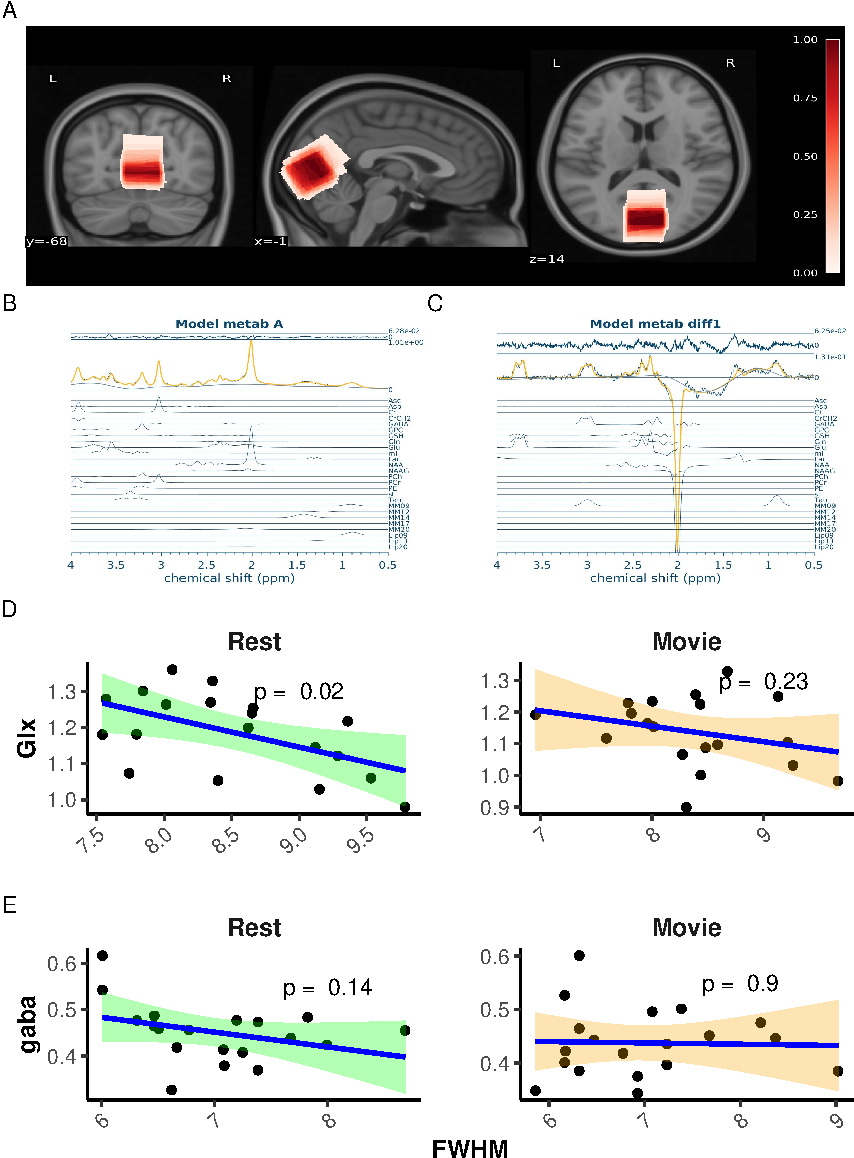
\includegraphics[keepaspectratio]{index_files/figure-pdf/fig-mrsquality-1.pdf}}

}

\caption{\label{fig-mrsquality}\textbf{MRS data quality} A) Average MRS
location. Overlay in red of the average voxel location across all
nineteen participants, from 0 (white) to 1 (dark red). Darker red
represents voxel locations shared by all participants, while white
represents voxel locations unique to participants. MRS voxels were
registered to MNI space and averaged. Underlay is T1w MNI152 at 0.5 mm
resolution. B) Sample Osprey sLASER Spectrum. Yellow spectrum indicates
overall model fit. Model fits for individual metabolites are shown in
blue below overall fit. C) Sample Osprey MEGAPRESS Spectrum. Yellow
spectrum indicates overall model fit. Model fits for individual
metabolites are shown in blue below overall fit. D) Correlation plots of
Glx / tCr vs.~FWHM for rest (green) and movie (red). E) Correlation
plots of GABA+ / tCr vs.~FWHM for rest (green) and movie (red).}

\end{figure}%

A sample of the combined grey-matter and MRS voxel mask used to average
H values, along with a sample Hurst exponent map, and sample fits for H
calculation during rest can be found in Figure~\ref{fig-hurstsamp} A, B,
and C, respectively.

Mean FD was not correlated with H during rest (r = -0.33, p = 0.16 but
was moderately negatively correlated with H during movie watching (r =
-0.50, p = 0.03; see Figure~\ref{fig-hurstsamp} D).

\phantomsection\label{cell-fig-hurstsamp}
\begin{figure}[H]

\centering{

\pandocbounded{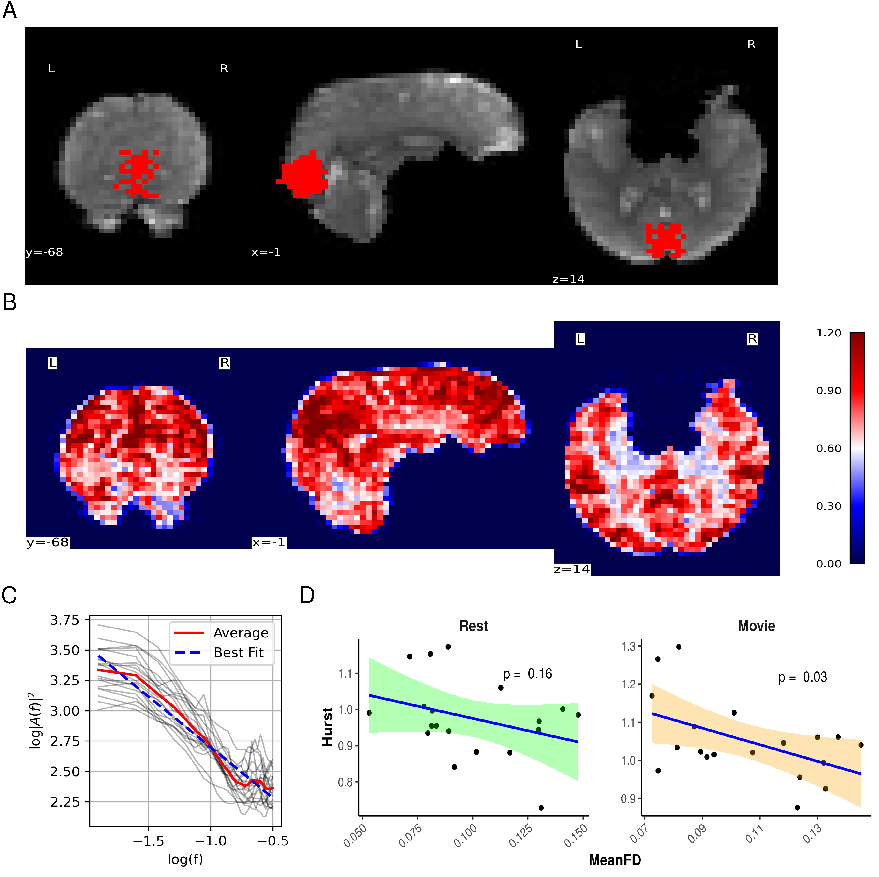
\includegraphics[keepaspectratio]{index_files/figure-pdf/fig-hurstsamp-1.pdf}}

}

\caption{\label{fig-hurstsamp}\textbf{fMRI data quality.} A) sample fMRI
grey-matter mask within the MRS voxel. Background: a sample coronal,
sagittal, and axial slice is displayed of the mean fMRI scan from the
rest acquisition. Foreground: the greymatter/MRS mask used to calculate
mean H. B) Sample H map for whole brain. Coronal, sagittal, and axial
views of are shown, colour-coded by H values. Colour-coding shows
evident tissue differentiation by H value (i.e., gray matter (red),
white matter (light red), and cerebrospinal fluid (white)). C) Sample
PSD spectrum. All participants' PSD spectrums during rest are plotted
using light grey lines. Mean PSD is plotted in solid red Mean linear
regression line is plotted in dashed blue. H for each participant was
calculated from the slope of their mean linear regression line. D)
Correlation plots of H vs.~meanFD for rest (green) and movie (orange).}

\end{figure}%

\subsection{Relationship between H and
E:I}\label{relationship-between-h-and-ei}

Mean ± sd of metabolites, E:I, and H during rest and movie are reported
in Table~\ref{tbl-results}. Boxplots between rest and movie can be seen
in Figure~\ref{fig-results}. Neither Glx nor GAB+ were different between
movie and rest conditions. E:I ratio did not change between conditions
either. H was found to be greater during movie watching than rest.

\begin{longtable}[]{@{}llll@{}}
\caption{\textbf{Summary of main
results}}\label{tbl-results}\tabularnewline
\toprule\noalign{}
& Rest & Movie & p-value \\
\midrule\noalign{}
\endfirsthead
\toprule\noalign{}
& Rest & Movie & p-value \\
\midrule\noalign{}
\endhead
\bottomrule\noalign{}
\endlastfoot
\textbf{Glx / tCr} & 1.19 ± 0.11 & 1.14 ± 0.11 & 0.09 \\
\textbf{GABA+ / tCr} & 0.45 ± 0.06 & 0.44 ± 0.06 & 0.50 \\
\textbf{E:I Ratio} & 2.68 ± 0.49 & 2.65 ± 0.45 & 0.82 \\
\textbf{H} & 0.98 ± 0.98 & 1.05 ± 1.05 & \textless{} 0.01 \\
\end{longtable}

\phantomsection\label{cell-fig-results}
\begin{figure}[H]

\centering{

\pandocbounded{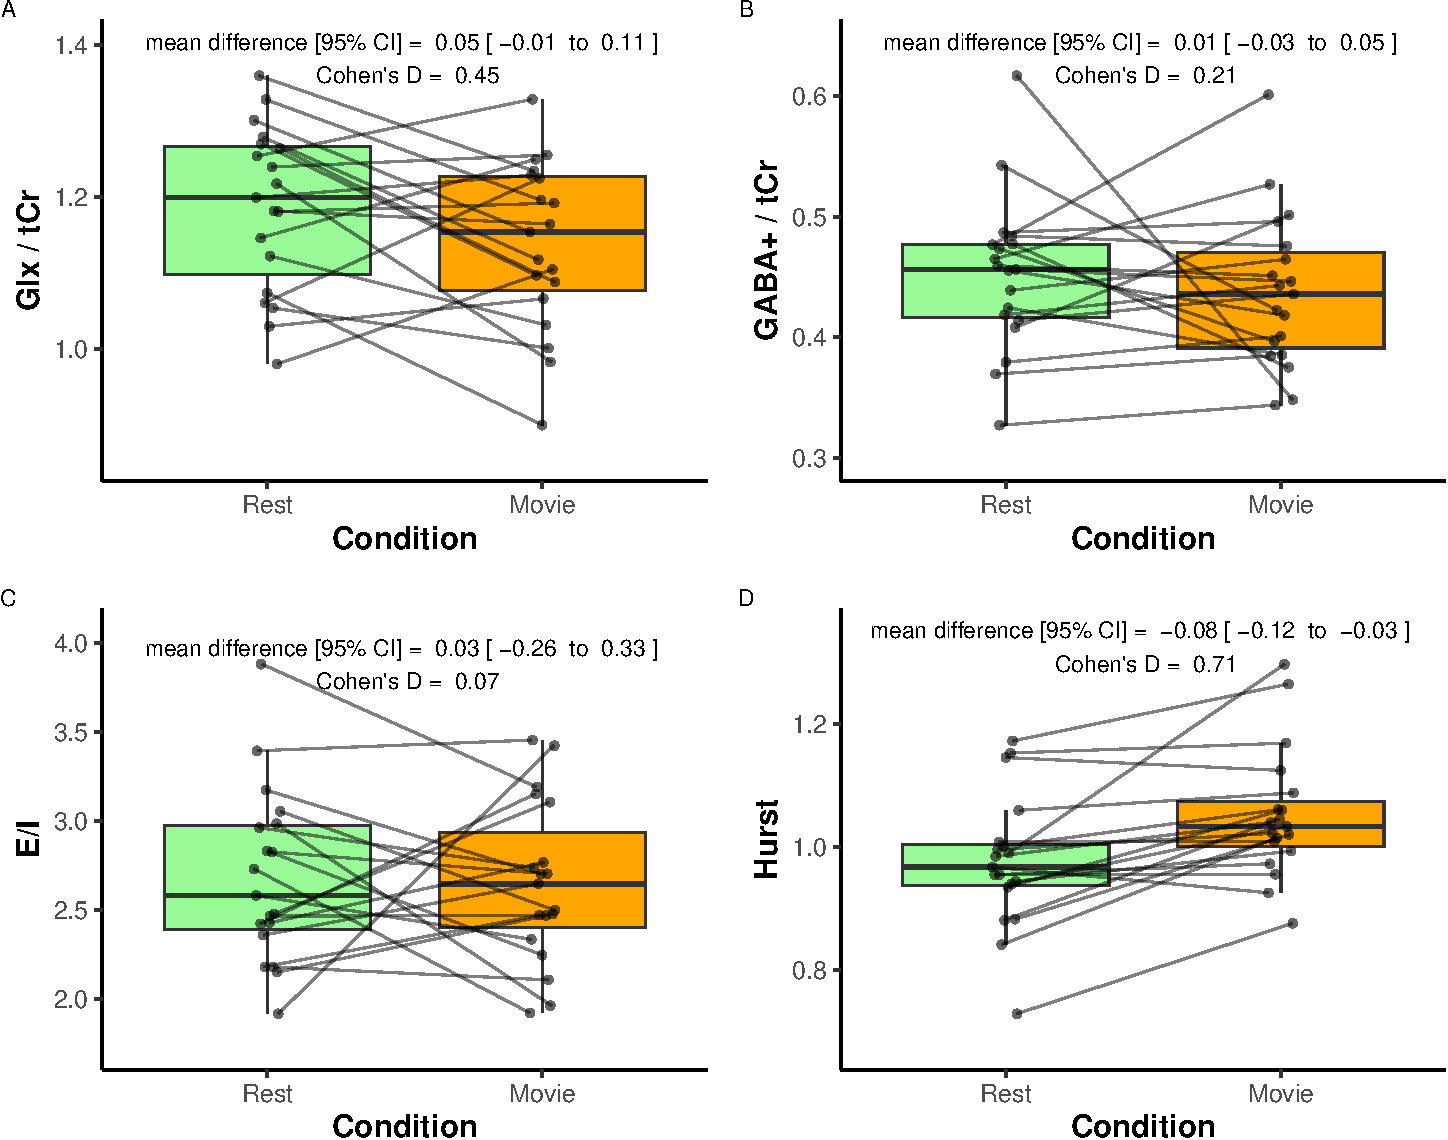
\includegraphics[keepaspectratio]{index_files/figure-pdf/fig-results-1.pdf}}

}

\caption{\label{fig-results}\textbf{Paired comparison of metabolite
values during rest (green) and movie (orange) conditions.} A) Glx / tCr;
B) GABA+ / tCr; and C) E:I. Paired dots represent the same participant
across conditions. Mean difference with 95\% confidence intervals, and
as Cohen's D are reported at the top of each plot.}

\end{figure}%

H was not found to correlate with Glx, GABA+, or E:I, during rest or
movie (Figure~\ref{fig-correlations}).

\phantomsection\label{cell-fig-correlations}
\begin{figure}[H]

\centering{

\pandocbounded{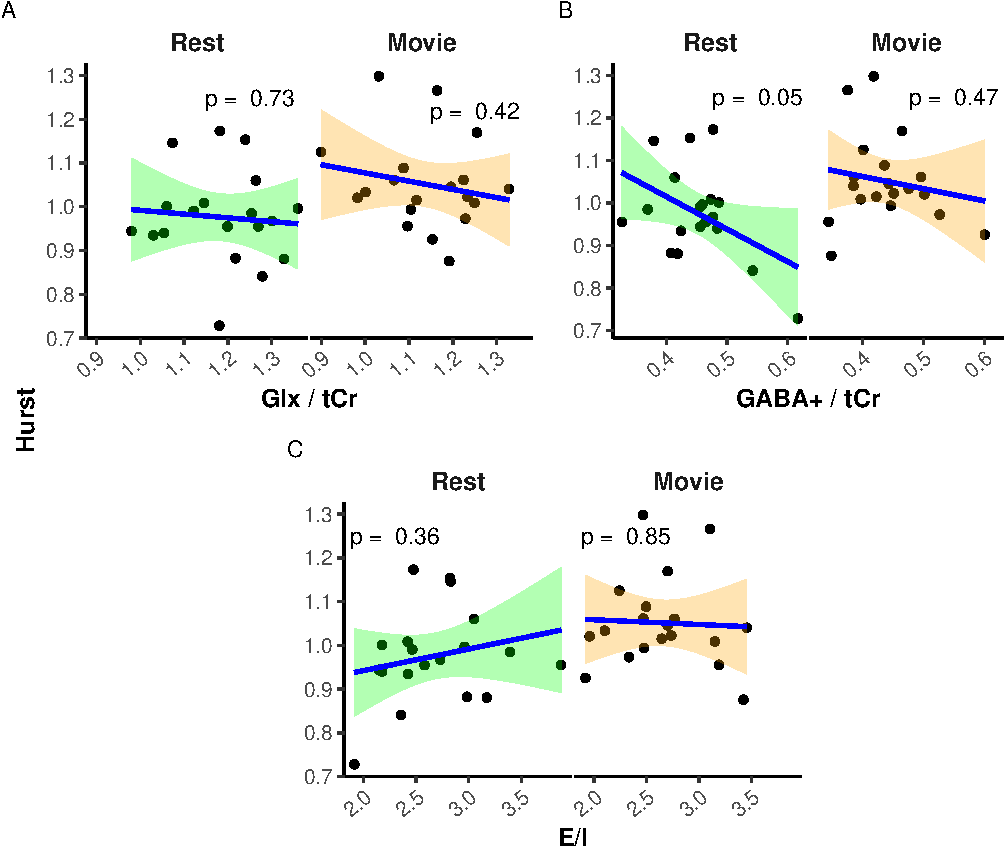
\includegraphics[keepaspectratio]{index_files/figure-pdf/fig-correlations-1.pdf}}

}

\caption{\label{fig-correlations}\textbf{Scatter plots of H
vs.~metabolites.} A) Glx / tCr; B) GABA+ / tCr; and C) E:I. Rest is in
green, while movie is in orange. p-values are reported at the top of
each plot.}

\end{figure}%

To ensure that meanFD and FWHM were not confounding our results, we also
ran a linear mixed-effects model with H as dependent variable, Glx/GABA+
as primary predictor of interest, and meanFD, FWHM(Glx), and FWHM(GABA+)
as covariates, Condition (rest vs.~movie) as fixed effects, and subjects
as random effects:

\[
\mathrm{H} \sim \frac{\mathrm{Glx}}{\mathrm{GABA+}} + \mathrm{meanFD} + \mathrm{FWHM_{Glx}} + \mathrm{FWHM_{GABA+}} + \mathrm{Condition} + (1 | \mathrm{Subject})
\]

The model's total explanatory power was substantial (conditional
r\textsuperscript{2} = 0.69), with fixed effects alone (marginal
r\textsuperscript{2}) equal to 0.19. The model's intercept,
corresponding to EI = 0, Condition = Movie, FWHMs\_Glx\_ = 0,
FWHM\_GABA+\_ = 0 and meanFD = 0, was 0.98 (95\% CI {[}0.41, 1.56{]},
t(30) = 3.34, p = 0.002). Within this model, only the effect of
Condition {[}Rest{]} was statistically significant (beta = -0.09, 95\%
CI {[}-0.13, -0.04{]}, t(30) = -3.99, p \textless{} 0.01).

\section{Discussion}\label{discussion}

We report here the first \emph{in vivo} human study of the E:I-H
relationship. An increase in H was observed during movie-watching as
compared to rest, indicating stronger long-range temporal dependencies
in BOLD activity during visual stimulation. No difference was found in
Glx, GABA+, nor Glx/GABA+ between rest and movie-watching. Furthermore,
no association was found between H and Glx, GABA+, nor Glx/GABA+.
Attempting to control for meanFD and FWHM using a linear mixed-effects
model did not alter these results.

Our finding that H increases during movie-watching compared to rest is
consistent with a previous study from our lab
\citep{campbellFractalBasedAnalysisFMRI2022}, which reported increased H
in the visual network (from Yeo's seven resting-state networks
\citep{thomasyeoOrganizationHumanCerebral2011}) during movie-watching
using data from the Human Connectome Project
\citep{vanessenHumanConnectomeProject2012}. While this increase in H is
consistent with our prior findings, other studies have reported
decreases in H during active tasks
\citep{heScaleFreePropertiesFunctional2011, churchillSuppressionScalefreeFMRI2016, ciuciuInterplayFunctionalConnectivity2014, barnesEndogenousHumanBrain2009}.
Our results suggest that the naturalistic, passive nature of
movie-watching elicits a different effect on H compared to more active
tasks. This is consistent with literature indicating distinct neural
responses and BOLD signal characteristics between conventional active
visual tasks and naturalistic passive visual stimuli
\citep{campbellFractalBasedAnalysisFMRI2022, hassonReliabilityCorticalActivity2010}.
Richer scaling properties (higher H) during movie-watching may support
the continuous perception of visual stimuli
\citep{campbellFractalBasedAnalysisFMRI2022}.

We found no changes in either Glx or GABA+ between conditions. Given
that no difference was observed for either metabolite, it is
unsurprising that E:I did not change either. This was unfortunate as our
study was designed to include two conditions in order to elicit changes
in H, Glx, and GABA+, aiming to confirm that our experiment induced
measurable alterations in these metrics. Establishing such changes would
have provided a foundation for directly examining the correlation
between H and the E/I ratio. However, because Glx and GABA+ did not show
significant changes between conditions, our main results are likely to
be met with doubt. Without evidence of condition-induced variations in
Glx and GABA+, it remains unclear whether the absence of correlation
reflects a true lack of association or insufficient sensitivity of our
measurement approach to detect changes in these metabolites.

A recent meta-analysis of Glu/Glx studies
\citep{pasantaFunctionalMRSStudies2023} reported a minimal task-induced
increase in Glu/Glx within the visual cortex; however, this finding was
not linked to any visual stimuli task, but rather to pain, learning, and
motor tasks. Additionally, many of the studies included in the review
were conducted at 7T, offering increased sensitivity for detecting
changes in Glu/Glx. Nonetheless, several studies have demonstrated
changes in Glu/Glx at 3T (e.g.,
\citep{gutzeitDifferentialNMRSpectroscopy2013, cleveAssessmentIntraInterregional2017, apsvalkaEventrelatedDynamicsGlutamate2015}).
Regarding our GABA+ findings, the same meta-analysis
\citep{pasantaFunctionalMRSStudies2023} reported no task-dependent
change in GABA within the visual cortex. This may be attributable to
technical difficulties associated with capturing GABA levels using MRS
at 3T due to its low concentration and signal overlap with more abundant
metabolites \citep{pasantaFunctionalMRSStudies2023}. Nevertheless, it is
worth noting that several studies have successfully reported changes in
GABA at 3T using different paradigms and/or regions of interest (e.g.,
\citep{floyer-leaRapidModulationGABA2006, sampaio-baptistaChangesFunctionalConnectivity2015, staggRoleGABAHuman2011}).

Another reason we may not have found changes in Glx or GABA+ may be due
to use of a block-design: collecting 24 minutes of rest data, then
collecting 24 minutes of movie-watching data. While a block design has
the advantage of a more robust metabolite quantification due to greater
signal averaging, brain homeostatis during these long blocks may lead to
an erasure of any real metabolic changes
\citep{mangiaMetabolicPathwaysActivitydependent2012, apsvalkaEventrelatedDynamicsGlutamate2015}.
Indeed, \citet{pasantaFunctionalMRSStudies2023} found the magnitude of
effect sizes were observed to be smaller for block designs than
event-related designs.

However, it may be possible that our results do support the idea that H
and E:I are not directly linked; at least not in a simple manner. This
is would perhaps not be surprising given the large disparity of findings
in the literature, especially with regard to the directionality and
linearity of the proposed E:I-Hurst relationship
\citep{liangExcitationInhibitionBalance2024, poilCriticalStateDynamicsAvalanches2012, lombardiBalanceExcitationInhibition2017, baumgartenCriticalExcitationinhibitionBalance2019, bruiningMeasurementExcitationinhibitionRatio2020, trakoshisIntrinsicExcitationinhibitionImbalance, gaoInferringSynapticExcitation2017}
(see Table~\ref{tbl-lit}). The heterogeneity across these E:I-Hurst
studies highlights the challenges of studying this phenomenon as well as
the complexity of any potential relationship between these two metrics.
It may be that, given the mixed-findings of these studies in combination
with our data, an E:I-Hurst relationship --- should it exist --- may
depend in part on how the data is collected. This could include
variables such as the experimental setup, sampling methods, or data
analysis techniques used. Further research is needed to elucidate the
true nature of any potential E:I-Hurst relationship and better
understand the complexities involved in studying this phenomenon.

\begin{longtable}[]{@{}
  >{\raggedright\arraybackslash}p{(\linewidth - 10\tabcolsep) * \real{0.1585}}
  >{\raggedright\arraybackslash}p{(\linewidth - 10\tabcolsep) * \real{0.1707}}
  >{\raggedright\arraybackslash}p{(\linewidth - 10\tabcolsep) * \real{0.1707}}
  >{\raggedright\arraybackslash}p{(\linewidth - 10\tabcolsep) * \real{0.1585}}
  >{\raggedright\arraybackslash}p{(\linewidth - 10\tabcolsep) * \real{0.1707}}
  >{\raggedright\arraybackslash}p{(\linewidth - 10\tabcolsep) * \real{0.1707}}@{}}
\caption{\textbf{Summary of methods for existing E:I-Hurst
studies}}\label{tbl-lit}\tabularnewline
\toprule\noalign{}
\begin{minipage}[b]{\linewidth}\raggedright
Citation
\end{minipage} & \begin{minipage}[b]{\linewidth}\raggedright
Study Type
\end{minipage} & \begin{minipage}[b]{\linewidth}\raggedright
H Data Type
\end{minipage} & \begin{minipage}[b]{\linewidth}\raggedright
H Calculation Method
\end{minipage} & \begin{minipage}[b]{\linewidth}\raggedright
E:I Type
\end{minipage} & \begin{minipage}[b]{\linewidth}\raggedright
E:I-Hurst Relationship
\end{minipage} \\
\midrule\noalign{}
\endfirsthead
\toprule\noalign{}
\begin{minipage}[b]{\linewidth}\raggedright
Citation
\end{minipage} & \begin{minipage}[b]{\linewidth}\raggedright
Study Type
\end{minipage} & \begin{minipage}[b]{\linewidth}\raggedright
H Data Type
\end{minipage} & \begin{minipage}[b]{\linewidth}\raggedright
H Calculation Method
\end{minipage} & \begin{minipage}[b]{\linewidth}\raggedright
E:I Type
\end{minipage} & \begin{minipage}[b]{\linewidth}\raggedright
E:I-Hurst Relationship
\end{minipage} \\
\midrule\noalign{}
\endhead
\bottomrule\noalign{}
\endlastfoot
Poil et al.~(2012)\citet{poilCriticalStateDynamicsAvalanches2012} &
Computational with in-house simulated model & Neuronal avalanche size &
Detrendend fluctuation analysis (DFA) & Structural: number of E-to-I
neurons & Inverse U \\
Bruining et
al.~(2020)\citet{bruiningMeasurementExcitationinhibitionRatio2020} &
Computational with model by Poil et al.~(2012); modified in-house &
Neuronal oscillation amplitude & DFA & Structural: number of E-to-I
synapses & Inverse U \\
Gao et al.~(2017)\citet{gaoInferringSynapticExcitation2017} &
Computational; in vivo in rats and macaques & Local field potential
(LFP) & PSD & Estimated from LFP & Positive linear \\
Lombardi et al.~(2017)\citet{lombardiBalanceExcitationInhibition2017} &
Computational with in-house model & Neuronal avalanche size & PSD &
Structural: number of E-to-I neurons & Negative linear \\
Trakoshis et
al.~(2020)\citet{trakoshisIntrinsicExcitationinhibitionImbalance} &
Computational with simulated data; in vivo in mice & fMRI BOLD signal &
Wavelet-based maximum likelihood method & E-to-I synaptic conductance &
Positive linear \\
\end{longtable}

Finally, it is also possible that while an E:I-Hurst relationship
exists, it is not observed within the visual cortex. This theory seems
plausible given that MRS studies of disrupted E:I, mostly conducted
within the context of adult autism spectrum disorder, have found changes
in E:I within other brain regions such as the anterior cingulate cortex,
frontal lobe, or temporal lobe \citep{ajramContribution1HMagnetic2019}.
Moreover, findings with reference to changes in excitatory or inhibitory
neurotransmitters within the visual cortex tend to be difficult to
capture, perhaps indicating that E:I shows less changes in this region
\citep{pasantaFunctionalMRSStudies2023}. However, this would suggest
that the E:I-H relationship would be region dependent, and therefore not
a generalizable theory as it is often portrayed.

\subsection{Limitations and Strengths}\label{limitations-and-strengths}

Beyond the limitations already mentioned (field strength, visual cortex,
passive task, block design), another limitation was our small sample
size. As this was a pilot study, 26 participants were initially scanned.
Once individuals were excluded for poor MRI quality, only 19
participants' data were analyzed. With this small sample size, it is
difficult to make conclusions about a concept as complex as the
E:I-Hurst relationship. We hope that by publishing our work, future
researchers can use our reported effect sizes to calculate potential
sample sizes. We would also like to list some of the strengths of our
study, which include: using sLASER (as opposed to PRESS), which has been
shown to have enhanced detection of complex multiplets such as Glu
\citep{wilsonMethodologicalConsensusClinical2019}; using the J-editing
sequence MEGA-PRESS for improved GABA detection
\citep{peekComprehensiveGuideMEGAPRESS2023}; using a large MRS voxel
size (\textasciitilde22 ml) as per consensus recommendations
\citep{peekBrainGABAGlutamate2020, choiSpectralEditing1H2021, linMinimumReportingStandards2021};
measuring H within the same region as our single-voxel MRS; and using
multi-echo fMRI for improved motion artifact regression
\citep{kunduMultiechoFMRIReview2017}.

\subsection{Lessons for Future
Researchers}\label{lessons-for-future-researchers}

Finally, we hope that by publishing our findings, we can provide some
guidance to future researchers. The following is a non-exhaustive list
of suggestions for future work:

\begin{itemize}
\tightlist
\item
  future studies should consider using ultra-high-field 7T MRI, which
  provides improved spectral resolution and more reliable detection of
  Glu and GABA compared to conventional 3T MRI;
\item
  examining paradigms that have consistently demonstrated alterations in
  these metabolites, such as pain studies, may enhance the likelihood of
  detecting changes in Glu and GABA
  \citep{archibaldMetaboliteActivityAnterior2020, cleveAssessmentIntraInterregional2017, gutzeitDifferentialNMRSpectroscopy2013}.
\item
  exploring brain regions beyond the visual cortex, such as the anterior
  cingulate cortex, which is commonly implicated in pain processing
  \citep{archibaldMetaboliteActivityAnterior2020, mullinsNovelTechniqueStudy2005, gussewTimeresolvedFunctional1H2010, gutzeitInsulaspecificResponsesInduced2011};
\item
  including a more diverse participant sample --- beyond healthy
  controls --- may help capture a wider range of H and E:I values,
  potentially improving sensitivity to metabolite-related changes;
\item
  increasing sample size in order to detect small effect sizes;
\item
  using an event-related design, as opposed to the block design we used,
  may provide more sensitivity to detecting rapid and transient neural
  responses due to its ability to isolate specific events within the
  scan session \citep{mullinsTheoryFunctionalMagnetic2018}. However, see
  \citet{pasantaFunctionalMRSStudies2023} for a longer discussion and
  possible downsides to this approach;
\item
  and finally, using a combined fMRI-MRS sequence
  \citep{ipCombinedFMRIMRSAcquires2017, dwyerSimultaneousMeasurementBOLD2021}
  to measure BOLD and Glu/GABA near-simultaneously.
\end{itemize}

Together, these considerations may help in overcoming the limitations
observed in the present study and contribute to a clearer understanding
of the potential relationship between E:I and H.

\section{Conclusion}\label{conclusion}

In conclusion, our findings do not support a relationship between H and
E:I in the visual cortex either during rest or during movie-watching at
3T in humans. In addition, while we found a task-related change in H, we
did not find any changes in Glu, GABA, or E:I between movie and rest.
Comparing our findings to the broader literature, E:I balance may be too
subtle to be detected with conventional 3T MRS methods. With regards to
the broader E:I-Hurst relationship, we similarly suggest that either
this relationship is insufficiently captured with our methods, or that
the relationship between these two variables may be more complex than
originally envisaged --- perhaps they are not directly related, but
rather connected through other mediating variables in a non-linear
fashion. To our knowledge, this is the first \emph{in vivo} human study
to test for this relationship. It is our hope that as the literature
grows, more authors will examine this relationship with respect to other
brain regions and using other methods, and will use the lessons learned
in this study to inform their own. Hopefully then it will be possible to
corroborate findings to probe the complex relationships that may exist
with regards to H and E:I in the human brain.

\section*{Data availability
statement}\label{data-availability-statement}
\addcontentsline{toc}{section}{Data availability statement}

All code used in this paper is available at
\href{https://github.com/WeberLab/EI_Hurst_Analysis}{github.com/WeberLab/EI\_Hurst\_Analysis}.
The data used in this paper is available by contacting the author. The
manuscript was written in a `reproducible manner'. The entire
manuscript, including statistics reported, figures, and tables, can be
reproduced here:
\href{https://weberlab.github.io/EI_Hurst_Manuscript/}{weberlab.github.io/EI\_Hurst\_Manuscript/}

\section*{Competing interests}\label{competing-interests}
\addcontentsline{toc}{section}{Competing interests}

The authors declare they have no known competing interests.

\section*{Author contributions}\label{author-contributions}
\addcontentsline{toc}{section}{Author contributions}

LS performed data curation, formal analysis, investigation, software,
visualization, and wrote the original draft. AMW performed,
conceptualization, data curation, formal analysis, funding acquisition,
investigation, methodology, project administration, resources,
supervision, validation, visualization, and writing - review \& editing.

\section*{Acknowledgements}\label{acknowledgements}
\addcontentsline{toc}{section}{Acknowledgements}

The work presented in this paper was supported in part by

\section*{References}\label{references}
\addcontentsline{toc}{section}{References}

\renewcommand{\bibsection}{}
\bibliography{EIHurst.bib}





\end{document}
